\documentclass[11pt,a4paper]{article}

\usepackage[utf8]{inputenc}
\usepackage[T1]{fontenc}
\usepackage{amsmath,amssymb,amsthm}
\usepackage{mathtools}
\usepackage{geometry}
\geometry{margin=2.4cm}
\usepackage{enumitem}
\usepackage{booktabs}
\usepackage{hyperref}
\hypersetup{colorlinks=true,linkcolor=blue!60!black,citecolor=blue!60!black,urlcolor=blue!60!black}
\usepackage{xcolor}
\usepackage{graphicx}
\graphicspath{{figures/}}

\theoremstyle{plain}
\newtheorem{theorem}{Theorem}[section]
\newtheorem{proposition}[theorem]{Proposition}
\newtheorem{lemma}[theorem]{Lemma}
\newtheorem{corollary}[theorem]{Corollary}
\newtheorem{remark}[theorem]{Remark}
\newtheorem{definition}[theorem]{Definition}
\newtheorem{assumption}[theorem]{Assumption}
\newtheorem{example}[theorem]{Example}

\newcommand{\R}{\mathbb{R}}
\newcommand{\CoP}{\mathrm{CoP}}
\newcommand{\tr}{\operatorname{tr}}
\newcommand{\diag}{\operatorname{diag}}
\newcommand{\LS}{\mathcal{L}}
\newcommand{\comment}{\textcolor{red}}

\title{\textbf{Torsional friction in planar contact}}
\author{Sébastien Kleff\\[2pt]
\small\texttt{sk8001@nyu.edu}}
\date{\today}

\begin{document}
\maketitle


\begin{abstract}
Tactile sensors are widely used to detect slip, but much less is known about what can actually be inferred about frictional contact limits from tactile measurements. This question matters because detecting that slip is occurring or imminent is not the same as knowing which tangential and torsional loads the contact can still support. That distinction is important for control design. In this report, we study this question for a single planar contact patch under quasi-static Coulomb friction. We first show that coarse normal force information, consisting of the total normal force and center of pressure, is generally insufficient to determine the admissible tangential wrench set: two contacts can have the same total normal force and CoP while supporting different combinations of tangential force and torsional moment. We then study what can still be inferred from partial measurements. In particular, we derive upper and lower bounds on the admissible wrench set from coarse measurements and from spatially distributed taxel-wise normal forces. The latter provide tighter bounds by reducing the ambiguity on how the normal force is distributed over the contact patch.
\end{abstract}

\section{Introduction}
Modern tactile sensors provide rich local information about contact pressure, shape, and deformation. Yet tactile features used for control are often selected mainly from empirical performance, for example contact pose, resultant force, image features, or local pressure measurements. A more basic question is less often made explicit: given a particular tactile measurement, what can actually be inferred about the physical interaction at the contact?
We study this question in the setting of a rigid planar contact patch under Coulomb friction. Rather than trying to characterize every possible tactile signal or manipulation task, we focus on one concrete control-relevant quantity: the set of tangential forces and torsional moments that the contact can support without violating the friction model.
The key difficulty is that this admissible wrench set depends on how the normal load is distributed over the patch. Coarse measurements such as the total normal force and center of pressure constrain this load distribution, but do not determine it uniquely. Spatial tactile measurements provide additional information and therefore reduce this ambiguity.
The objective of this report is to make this relationship explicit. We ask \textbf{how the admissible frictional wrench set can be bounded from different levels of normal force information}, from total force and CoP to spatially distributed taxel-wise forces, \textbf{without requiring the full normal pressure field}.
This short version states the main results without proofs. Proofs and technical conditions (taxel boundaries, attainment of the bounds) are given in the full report.

\section{Preliminaries (measures)}
\label{sec:measure-preliminaries}

We briefly introduce the measure-theoretic notation used in the following.
Only the notions needed for the contact model are recalled here; standard reference
is \cite{evans2015measure}.

\subsection{Force as a measure.}
Let $P\subset\mathbb R^2$ denote the contact patch, equipped with its Borel
$\sigma$-algebra $\mathcal B(P)$. A \textit{nonnegative measure} $\nu_N:\mathcal B(P)\rightarrow[0,+\infty]$ assigns to every measurable subset $A\subseteq P$ a nonnegative scalar $\nu_N(A)$, and is countably additive, i.e. for any pairwise disjoint measurable sets $A_i \subseteq P$,
\begin{align}
\nu_N\left(\bigcup_i A_i\right) =\sum_i \nu_N(A_i).
\end{align}
In the present context, $\nu_N$ represents the (spatially distributed) normal force, i.e. $\nu_N(A)$ is the normal force carried by the region A. Hence $\nu_N(A)$ has units of force (N), and the resultant normal force is $f_N=\nu_N(P)$. We restrict attention to \textit{finite nonnegative Radon measures}, denoted $\nu_N\in\mathcal M_+(P)$. Informally, a Radon measure is a "well-behaved" measure. In particular, on the compact sets considered here, it is finite and its value on measurable sets can be approximated from compact subsets. For our purpose, it essentially means that our measure does not assign an infinite force to $P$ and it can represent either the force induced by an ordinary pressure field or an idealized concentrated point/line load.

We represent the tangential force by an $\mathbb R^2$-valued finite Radon measure $\nu_T=(\nu_{T,1},\nu_{T,2})$ where each component $\nu_{T,i}$ is a finite signed Radon measure on $P$. Thus, for every measurable region $E\subseteq P$, the resultant tangential force carried by $E$ is
\begin{align}
    \nu_T(E)
    =
    \begin{bmatrix}
    \nu_{T,1}(E)\\
    \nu_{T,2}(E)
    \end{bmatrix}
    \in\mathbb R^2,
\end{align}

\subsection{Area measure and pressure fields.}
Let $dA$ denote the usual area element on the planar patch $P$.
A \textit{normal pressure field} is a nonnegative function $\rho_N:P\rightarrow\mathbb R_+$ with units of force per unit area. If $\rho_N\in L^1_+(P)$, which simply means that $\rho_N$ has finite integral over $P$
\begin{align}
\rho_N(x)\ge 0\quad\text{a.e.},
\qquad
\int_P \rho_N(x)\,dA<\infty.
\end{align}
then it defines a finite normal force measure: the force carried by any region $E\subseteq P$ is given by
\begin{align}
\nu_N(E) = \int_E \rho_N(x)\,dA.
\end{align}
which we also write equivalently as $d\nu_N(x)=\rho_N(x)\,dA$. In that case, $\rho_N$ is called the \textit{density} of the normal force measure $\nu_N$ with respect to area\footnote{More generally, the Radon-Nikodym theorem guarantees the existence of a density for measures under suitable assumptions, such as "absolute continuity" which means physically that a subset of zero area (e.g. a point or a line) carries zero normal force. See~\cite{evans2015measure}, Theorem 1.30, p. 50}. Not every normal force measure admits such a pressure field. For example the Dirac measure $\nu_N=f_N\delta_c$ represents an idealized normal force $f_N$ concentrated at the single point $c$. It cannot be represented by an ordinary pressure field over area. In this note we adopt the measure-theoretic language (instead of only $L_+^1$ densities) so that we cover both "classical" pressure fields and idealized concentrated loads.

This notation allows ordinary pressure fields and concentrated loads to be handled by the same integration equations. For a measurable scalar or vector function $g$, the integral 
\begin{align}
\int_P g(x)\,d\nu_N(x)
\end{align}
can be interpreted as a force-weighted spatial integral. 
Whenever $\nu_N$ admits a normal pressure field $\rho_N$,
\begin{align}
\int_P g(x)\,d\nu_N(x) = \int_P g(x)\rho_N(x)\,dA.
\end{align} 
For a Dirac measure,
\begin{align}
\int_P g(x)\,d(f_N\delta_c)(x) = f_Ng(c).
\end{align}

\subsection{Moments of the normal force measure.}
The zeroth moment of $\nu_N$ is its total measure,
\begin{align}
m_0(\nu_N) \triangleq \int_P 1\,d\nu_N = \nu_N(P) = f_N.
\end{align}
In the present mechanical interpretation, this is the \textit{resultant normal force}. The first moment is
\begin{align}
m_1(\nu_N) \triangleq \int_P x\,d\nu_N(x)\in\mathbb R^2.
\end{align}
If $f_N>0$, the \textit{center of pressure} is the normalized first moment, 
\begin{align} 
c[\nu_N] &\triangleq \frac{m_1(\nu_N)}{m_0(\nu_N)} \\
         & = \frac{1}{f_N} \int_P x\,d\nu_N(x).
\end{align}
Hence knowing the total normal force and the center of pressure is equivalent to knowing the zeroth and first moments of the normal force measure $m_0(\nu_N)=f_N, m_1(\nu_N)=f_Nc[\nu_N]$. 

\paragraph{Barycenters and local CoPs.}
More generally, the \textit{barycenter} of a nonnegative measure $\nu$ carried by a set $E$ with $\nu(E)>0$ is its normalized first moment
$\frac{1}{\nu(E)}\int_E x\,d\nu(x)$. For the normal force measure on $P$, the barycenter is the CoP, $c[\nu_N]$. For the restriction of $\nu_N$ to a
subset $E\subseteq P$, such as a taxel, it is the \textit{local CoP} of the normal force carried by $E$.

\section{Problem formulation}
\subsection{Planar contact model}

Assume that the planar contact patch $P\subset\mathbb R^2$ is compact and convex,
and let $\nu_N\in\mathcal M_+(P)$ and $\nu_T$ be the normal and tangential force
measures introduced above. We assume
\begin{align}
f_N=m_0(\nu_N)>0,
\end{align}
so that the center of pressure $c$ is well-defined. Since $P$ is convex and
$\nu_N$ is nonnegative, $c\in P$.
We further assume a known and spatially uniform Coulomb friction coefficient
$\mu>0$.
We impose Coulomb friction in measure form by requiring that there exists a
measurable density $\gamma_T:P\rightarrow\mathbb R^2$ of $\nu_T$ with respect
to $\nu_N$ such that
\begin{align}
\label{eq:coulomb_measure}
d\nu_T(x)=\gamma_T(x)\,d\nu_N(x),
\qquad
\|\gamma_T(x)\|_2\le\mu
\quad \nu_N\text{-a.e. on }P.
\end{align}
We call $\gamma_T$ the \textit{friction ratio field}. It can be interpreted as
the tangential force per unit normal force. 
The above condition expresses both that tangential friction force can only be carried where normal force is present
and that its local magnitude is bounded by $\mu$\footnote{In particular, $d\nu_T=\gamma_T\,d\nu_N$ implies
$\nu_T\ll\nu_N$.}. When $\nu_N$ admits the normal pressure field $\rho_N$ introduced above, i.e. $d\nu_N=\rho_N\,dA$, the tangential force measure also admits a density with respect to area,
\begin{align}
\rho_T(x)=\gamma_T(x)\rho_N(x),
\end{align}
called the \textit{tangential traction field}. The measure-form Coulomb condition then reduces to the classical local condition
\begin{align}
\label{eq:coulomb_local}
\|\rho_T(x)\|_2\le\mu\rho_N(x)
\qquad \text{a.e. on }P.
\end{align}
We define the \textit{resultant tangential force} and \textit{resultant torsional moment} about the center of pressure $c$ as
\begin{align}
f_T \triangleq \nu_T(P)
= \int_P\gamma_T(x)\,d\nu_N(x),
\qquad
\tau_N \triangleq
\int_P (x-c)\times\gamma_T(x)\,d\nu_N(x).
\end{align}
We finally define the skew-symmetric matrix
\begin{align}
J \triangleq
\begin{bmatrix}
0&-1\\
1&0
\end{bmatrix},
\end{align}
so that for $x,y\in\mathbb R^2$ $x\times y=(Jx)^\top y$

\begin{definition}[Admissible tangential wrench set]
    Define a normal force measure $\nu_N\in\mathcal M_+(P)$. We define \textit{admissible tangential wrench set} :
    \begin{align}
    \mathcal W(\nu_N)
    \triangleq
    \left\{
    (f_T,\tau_N)\in\mathbb R^2\times\mathbb R:
    \begin{array}{l}
    \exists\,\gamma_T:P\rightarrow\mathbb R^2
    \text{ measurable such that}\\
    \|\gamma_T(x)\|_2\le\mu
    \quad\nu_N\text{-a.e.},\\
    f_T=\displaystyle\int_P\gamma_T(x)\,d\nu_N(x),\\
    \tau_N=\displaystyle\int_P
    (x-c[\nu_N])\times\gamma_T(x)\,d\nu_N(x)
    \end{array}
    \right\}.
    \end{align}
    The set $\mathcal W(\nu_N)$ is a non-empty compact subset of $\R^3$ containing all resultant tangential wrenches (tangential force and torsional moment) that are compatible with the normal force measure $\nu_N$ and the local Coulomb friction condition~\eqref{eq:coulomb_measure}.
\end{definition}




\begin{proposition}[Support function of the admissible tangential wrench set]
    \label{prop:support}
    For any $\nu_N\in\mathcal M_+(P)$ and for every $q=(a,b)\in\mathbb R^2\times\mathbb R$, the support function of $\mathcal W(\nu_N)$ is
    \begin{align}
    h_{\mathcal W(\nu_N)}(q) = \mu \int_P \left\|a+bJ(x-c[\nu_N])\right\|_2\,d\nu_N(x).
    \end{align}
\end{proposition}
\begin{proof}
    By definition, $\forall q=(a,b)\in\R^2\times \R$
    \begin{align}
    h_{\mathcal W(\nu_N)}(q) =\sup_{(f_T,\tau_N)\in\mathcal W(\nu_N)}\left(a^\top f_T+b\tau_N\right).
    \end{align}
    For any friction ratio field $\gamma_T$
    \begin{align}
    a^\top f_T+b\tau_N=\int_P\left[a+bJ(x-c[\nu_N])\right]^\top\gamma_T(x)\,d\nu_N(x).
    \end{align}
    Using Cauchy--Schwarz and
    $\|\gamma_T(x)\|_2\le\mu$,
    \begin{align}
    a^\top f_T+b\tau_N\le\mu\int_P\left\|a+bJ(x-c[\nu_N])\right\|_2\,d\nu_N(x).
    \end{align}
    The bound is attained by choosing $\gamma_T(x)$ with magnitude $\mu$ and aligned with
    $a+bJ(x-c[\nu_N])$ whenever this vector is nonzero:
    \begin{align}
        \gamma_T^{\star}(x)= \begin{cases}
                \mu\frac{a + bJ(x-c[\nu_N])}{\|a + bJ(x-c[\nu_N])\|_2}~~&\text{if}~\|a + bJ(x-c[\nu_N])\|_2\neq 0\\
                0~~&\text{otherwise}
        \end{cases} 
    \end{align}
\end{proof}


\subsection{Measurement-conditioned support bounds}
\begin{table}[t]
    \centering
    \small
    \resizebox{\textwidth}{!}{\begin{tabular}{llll}
        \toprule
        Symbol & Meaning & Remark & Lives in \\
        \midrule
        $\nu_N$ 
        & normal force measure
        & true $\nu_N^\star$ is unknown
        & $\mathcal M_+(P)$
        \\
        $c[\nu_N]$
        & CoP induced by measure $\nu_N$
        & depends on $\nu_N$
        & $P\subset\mathbb R^2$
        \\
        $q=(a,b)$
        & wrench support direction
        & prescribed
        & $\mathbb R^2\times\mathbb R$
        \\
        $\mathcal M$
        & measurement operator
        & fixed by the sensing model
        & $\mathcal M_+(P)\rightarrow\mathbb R^r$
        \\
        $y$
        & measurement value 
        & observed data from $(\mathcal M,\nu_N)$
        & $\mathbb R^r$
        \\
        $\Pi_{\mathcal M}(y)$
        & all measures compatible with $y$
        & depends on $(\mathcal M,y)$
        & $\subseteq\mathcal M_+(P)$
        \\
        $\mathcal C_{\mathcal M}(y)$
        & CoPs compatible with $y$
        & depends on $(\mathcal M,y)$
        & $\subseteq P$
        \\
        $\underline h_{\mathcal M}(q;y)$
        & measurement-conditioned lower bound
        & depends on $(\mathcal M,y,q)$
        & $\mathbb R$
        \\
        $\overline h_{\mathcal M}(q;y)$
        & measurement-conditioned upper bound
        & depends on $(\mathcal M,y,q)$
        & $\mathbb R$
        \\
        \bottomrule
    \end{tabular}}
    \caption{Notations.}
    \label{tab:measurement_notation}
\end{table}

We focus here on the case where we do not know the \textit{true} force measure $\nu_N^\star$ but we have only access to some measurements of it (e.g. resultant normal force, CoP, etc.). 
The goal is to investigate what can be known about the support of $\mathcal W(\nu_N^\star)$ given partial measurements of $\nu_N^\star$. 
\begin{definition}[Measurement operator]\label{def:measurement_operator}
    We define a \textit{measurement operator} as a function $\mathcal M:\mathcal M_+(P)\rightarrow\mathbb R^r$. We assume that its components are linear integral measurements of the form
    \begin{align}
    \mathcal M(\nu_N) = 
    \begin{bmatrix}
    \displaystyle\int_P \phi_1(x)\,d\nu_N(x)\\
    \vdots\\
    \displaystyle\int_P \phi_r(x)\,d\nu_N(x)
    \end{bmatrix},\qquad \forall \nu_N \in \mathcal M_+(P)
    \end{align}
    where the prescribed measurable functions
    $\phi_j:P\rightarrow\mathbb R$ are called the \textit{measurement functions}.
    In the following, we denote a measurement value (or observation) induced by the (unknown) true force measure $\nu_N^\star$ as $y = \mathcal M(\nu_N^\star) \in\mathbb R^r$.
\end{definition}

\begin{definition}[Measurement-compatible normal force family]
    Given a measurement operator $\mathcal M:\mathcal M_+(P)\rightarrow\mathbb R^r$ and the observation $y\in\R^r$, we define the set of \textit{normal force measures that are compatible with observation $y$} 
    \begin{align}
    \Pi_{\mathcal M}(y) \triangleq\left\{\nu_N\in\mathcal M_+(P):\mathcal M(\nu_N)=y\right\}.
    \end{align}
    The set $\Pi_{\mathcal M}(y)$ contains all the normal force measures that are indistinguishable under measurement $y$. Note that this is the pre-image of $y$ through $\mathcal{M}$ : $\Pi_{\mathcal{M}(y)} = \mathcal{M}^{-1}[\{y\}]$.
\end{definition}

\begin{assumption}
    \label{ass:positive_mass}
    From now on, we assume \(\forall \nu_N\in\Pi_{\mathcal M}(y)\), $\nu_N(P) >0$. Purpose: we restrict the measurement-compatible family to measures that have a well-defined CoP.
\end{assumption}

\begin{definition}[Set of measurement-compatible CoPs]\label{def:CM}
    We define
    \begin{align}
    \mathcal C_{\mathcal M}(y)
    \triangleq
    \left\{
    c[\nu_N]:
    \nu_N\in\Pi_{\mathcal M}(y)
    \right\}
    \end{align}
    as the set of CoPs compatible with the observation $y \in \mathbb{R}^r$.    
\end{definition}

Given an observation $y$ of the unknown true force measure $\nu_N^\star$, we can compute measurement-conditioned lower/upper bounds on the support function $h_{\mathcal W(\nu_N^\star)}$ by optimizing over $\Pi_{\mathcal M}(y)$. 

\begin{definition}[Measurement-conditioned support bounds]\label{def:measurement_support_bounds}
Let $\mathcal M:\mathcal M_+(P)\rightarrow\mathbb R^r$ be a measurement operator as defined above and let $y=\mathcal M(\nu_N^\star)$ denote the observation induced by the unknown true normal force measure $\nu_N^\star$. For a wrench direction $q\in\mathbb R^2\times\mathbb R$, we define the \textit{measurement-conditioned bounds in direction $q$}:
\begin{align}
    \label{eq:def_mea_bounds}
    \underline h_{\mathcal M}(q;y)
    &\triangleq
    \inf_{\nu_N\in\Pi_{\mathcal M}(y)}
    h_{\mathcal W(\nu_N)}(q),\\
    \overline h_{\mathcal M}(q;y)
    &\triangleq
    \sup_{\nu_N\in\Pi_{\mathcal M}(y)}
    h_{\mathcal W(\nu_N)}(q).
\end{align}
\end{definition}


\begin{remark}[How to use the bounds $\underline h_{\mathcal M}(q;y), \overline h_{\mathcal M}(q;y)$]
    \label{rem:use_bounds}
    A practical consequence of knowing the bounds is that we can test the slip feasibility of a candidate tangential wrench $w$: guaranteed feasible if $\forall q,~\langle q,w\rangle \le \underline h_{\mathcal M}(q;y)$.
    Conversely, if $\exists q,~\langle q,w\rangle >\overline h_{\mathcal M}(q;y)$, then $w$ is infeasible for every normal force measure compatible with the measurement $y$\footnote{Because all support functions are positively homogeneous in $q$, it is sufficient in practice to search over one normalized representative of each nonzero ray. After fixing a consistent scaling between force and torque coordinates, one may for instance impose $\|q\|_2=1$.}.
\end{remark}


\begin{remark}[Relation with inner/outer wrench sets]
    \label{rem:inner_outer}
    We can relate the bounds of Definition~\ref{def:measurement_support_bounds} to outer/inner approximations of the admissible wrench set
    \begin{align}
        \mathcal W^+(y)
        &\triangleq
        \bigcup_{\nu_N\in\Pi_{\mathcal M}(y)}\mathcal W(\nu_N),
        &
        \mathcal W^-(y)
        &\triangleq
        \bigcap_{\nu_N\in\Pi_{\mathcal M}(y)}\mathcal W(\nu_N).
        \end{align}
    Then $h_{\mathcal W^+(y)}(q) =\overline h_{\mathcal M}(q;y)$ and $h_{\mathcal W^-(y)}(q) \le\underline h_{\mathcal M}(q;y)$ (equality need not hold for the inner set). Nevertheless, the lower bound characterizes the inner set exactly through
    \begin{align}
        \mathcal W^-(y)
        =
        \left\{
        w:\,
        \langle q,w\rangle
        \le
        \underline h_{\mathcal M}(q;y)
        \quad \forall q
        \right\}.
    \end{align}
\end{remark}

Computing the bounds of Definition~\ref{def:measurement_support_bounds} is difficult in general as it leads to a nonlinear optimization problem over measurement-compatible measures:
\begin{align}
    \underline h_{\mathcal M}(q;y)
    &=
    \inf_{\nu_N\in\Pi_{\mathcal M}(y)}
    \mu
    \int_P
    \left\|
    a+bJ\left(
    x-
    c[\nu_N]
    \right)
    \right\|_2
    \,d\nu_N(x),
    \label{eq:general_nonlinear_lower}
    \\
    \overline h_{\mathcal M}(q;y)
    &=
    \sup_{\nu_N\in\Pi_{\mathcal M}(y)}
    \mu
    \int_P
    \left\|
    a+bJ\left(
    x-
    c[\nu_N]
    \right)
    \right\|_2
    \,d\nu_N(x).
    \label{eq:general_nonlinear_upper}
\end{align}
The objective is nonlinear in the measure $\nu_N$ since the integrand depends
on it through $c[\nu_N]$. Hence, this is not a standard Generalized
Moment Problem (GMP)~\cite{lasserre2010moments}. The next subsection collects the
generic properties of \eqref{eq:general_nonlinear_lower}--\eqref{eq:general_nonlinear_upper}
that are used for all the measurement operators studied afterwards.

\subsection{General structure of the bounds}
\label{sec:general_structure}

For $q=(a,b)\in\R^2\times\R$ and a reference point $c\in\R^2$, we write
\begin{align}
    \label{eq:def_g}
    g(x;q,c)\triangleq\left\|a+bJ(x-c)\right\|_2,
\end{align}
so that, by Proposition~\ref{prop:support},
$h_{\mathcal W(\nu_N)}(q)=\mu\int_P g(x;q,c[\nu_N])\,d\nu_N(x)$.
Since $x\mapsto g(x;q,c)$ is convex, Jensen's inequality gives a lower bound valid for every normal force measure,
\begin{align}
    \label{eq:universal_lower}
    h_{\mathcal W(\nu_N)}(q)\ge\mu\,\nu_N(P)\,\|a\|_2.
\end{align}
Two structural facts organize the rest of the report.

\begin{lemma}[CoP slicing]
\label{lem:cop_slicing}
    For $c\in\R^2$, let
    $\Pi_{\mathcal M}(y;c)\triangleq\left\{\nu_N\in\Pi_{\mathcal M}(y):\int_P(x-c)\,d\nu_N(x)=0\right\}$
    be the compatible measures whose CoP is $c$. Then
    $\Pi_{\mathcal M}(y)=\bigcup_{c\in\mathcal C_{\mathcal M}(y)}\Pi_{\mathcal M}(y;c)$, and
    \begin{align}
        \underline h_{\mathcal M}(q;y)
        &=
        \inf_{c\in\mathcal C_{\mathcal M}(y)}
        \;
        \inf_{\nu_N\in\Pi_{\mathcal M}(y;c)}
        \mu\int_P
        g(x;q,c)\,d\nu_N(x),
        \label{eq:parametric_gmp_lower}
        \\
        \overline h_{\mathcal M}(q;y)
        &=
        \sup_{c\in\mathcal C_{\mathcal M}(y)}
        \;
        \sup_{\nu_N\in\Pi_{\mathcal M}(y;c)}
        \mu\int_P
        g(x;q,c)\,d\nu_N(x).
        \label{eq:parametric_gmp_upper}
    \end{align}
    For a fixed $c$, the inner problems are linear in $\nu_N$ under linear moment constraints, i.e. GMPs.
    In particular, if $\mathcal C_{\mathcal M}(y)=\{c\}$ is a singleton, the outer optimization disappears and
    both bounds are GMPs.
\end{lemma}

\begin{lemma}[Monotonicity with respect to information]
\label{lem:monotone}
    Let $(\mathcal M,y)$ and $(\mathcal M',y')$ be two measurement operators and observations such that
    $\Pi_{\mathcal M'}(y')\subseteq\Pi_{\mathcal M}(y)$. Then $\mathcal C_{\mathcal M'}(y')\subseteq\mathcal C_{\mathcal M}(y)$ and,
    for every $q\in\R^2\times\R$ and every $\nu_N\in\Pi_{\mathcal M'}(y')$,
    \begin{align}
        \underline h_{\mathcal M}(q;y)
        \le
        \underline h_{\mathcal M'}(q;y')
        \le
        h_{\mathcal W(\nu_N)}(q)
        \le
        \overline h_{\mathcal M'}(q;y')
        \le
        \overline h_{\mathcal M}(q;y).
    \end{align}
    This applies in particular to $\nu_N=\nu_N^\star$ when $y'=\mathcal M'(\nu_N^\star)$.
\end{lemma}

Table~\ref{tab:measurement_cases} summarizes the measurement operators studied in the remainder of the report and the structure of the resulting problems,
and Figure~\ref{fig:measurements} illustrates what each of them observes.
\begin{figure}[t]
    \centering
    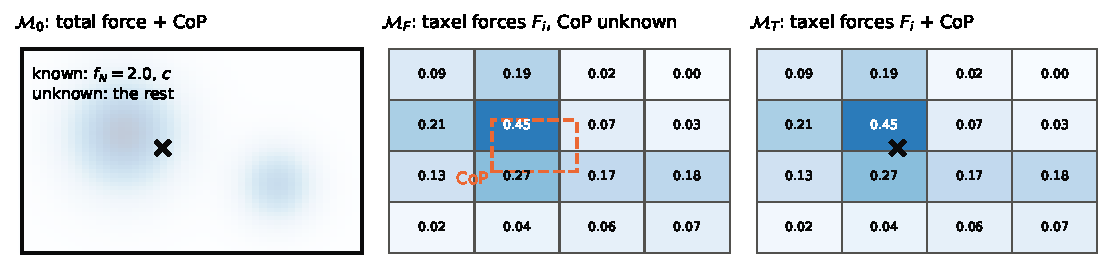
\includegraphics[width=\textwidth]{measurements}
    \caption{What each measurement operator observes for the same contact ($4\times4$ taxels). $\mathcal M_0$: only $f_N$ and the CoP, the pressure
    distribution (faded) is unknown. $\mathcal M_F$: the taxel forces $F_i$ (cells filled with the mean pressure $F_i/|P_i|$), the CoP is only known to lie
    in $\mathcal C_{\mathcal M_F}(y_F)$ (dashed, Proposition~\ref{prop:cop_taxel}). $\mathcal M_T$: taxel forces and CoP.}
    \label{fig:measurements}
\end{figure}
\begin{table}[t]
    \centering
    \small
    \resizebox{\textwidth}{!}{\begin{tabular}{lllll}
        \toprule
        Measurement & Observed data & Compatible CoP set & Lower bound & Upper bound \\
        \midrule
        $\mathcal M_0$ (Sec.~\ref{sec:M0})
        &
        $y_0=(f_N,f_Nc)$
        &
        $\{c\}$
        &
        closed form
        &
        LP (polygonal $P$)
        \\[1mm]
        $\mathcal M_T$ (Sec.~\ref{sec:MT})
        &
        $y_T=(y_0,y_F)$
        &
        $\{c\}$
        &
        convex (SOCP)
        &
        LP (polygonal taxels)
        \\[1mm]
        $\mathcal M_F$ (Sec.~\ref{sec:MF})
        &
        $y_F=(F_1,\ldots,F_r)$
        &
        $\displaystyle\sum_{i=1}^r\frac{F_i}{f_N}P_i$
        &
        convex (SOCP)
        &
        nonconvex: $\max_{c}$ of $\mathcal M_T$ LPs
        \\
        \bottomrule
    \end{tabular}}
    \caption{Measurement operators, compatible CoP sets and structure of the resulting bounds.}
    \label{tab:measurement_cases}
\end{table}
We next specialize \eqref{eq:general_nonlinear_lower}--\eqref{eq:general_nonlinear_upper} by increasing difficulty:
the CoP is first measured, with coarse (Section~\ref{sec:M0}) and then taxel-wise (Section~\ref{sec:MT}) force information.
It is then unknown (Section~\ref{sec:MF}). The tightening of the bounds as information is added is studied in Section~\ref{sec:refinement}.

\section{$\mathcal{M}_0$ case (coarse measurement)}
\label{sec:M0}

We first assume that the available measurements consist only of the resultant normal force $f_N$ and the CoP $c$.
\textit{Known:} $P$, $\mu$, $f_N$ and $c$. \textit{Unknown:} how $\nu_N^\star$ is distributed over $P$.
Since the CoP is measured, Lemma~\ref{lem:cop_slicing} shows that both bounds are GMPs. We compute them explicitly and show
that this partial information is generally not enough to determine the admissible tangential wrench set.

\begin{definition}[Coarse normal force measurement]\label{def:coarse_measurement}
    Given the true (unknown) normal force measure $\nu_N^\star\in\mathcal M_+(P)$,
    we define the coarse measurement as its zeroth and first moments
    \begin{align}
    y_0 = \mathcal M_0(\nu_N^\star) \triangleq \left(\int_P d\nu_N^\star(x),\;\int_P x\,d\nu_N^\star(x)\right) = (f_N,f_Nc[\nu_N^\star]),
    \end{align}
    i.e. the measurement functions are $\phi_1(x)=1$, $\phi_2(x)=x_1$, $\phi_3(x)=x_2$. The set of compatible CoPs is the singleton $\mathcal C_{\mathcal M_0}(y_0)=\{c[\nu_N^\star]\}$.
\end{definition}

\begin{theorem}[Exact coarse lower bound]
\label{thm:coarse_lower}
    Let $c=c[\nu_N^\star]$. Given the coarse observation $y_0=(f_N, f_Nc)$, for any $q=(a,b)\in\mathbb R^2\times\mathbb R$,
    \begin{align}
            \boxed{\underline h_{\mathcal M_0}(q;y_0) = \mu f_N\|a\|_2}
    \end{align}
    The value follows from \eqref{eq:universal_lower}, and is attained by the point load $f_N\delta_c$.
\end{theorem}

As an immediate consequence, setting $a=0$ shows that the coarse measurement does not guarantee any torsional capacity, i.e. $\underline h_{\mathcal M_0}((0,b);y_0)=0$.

\begin{theorem}[Coarse upper bound]
\label{cor:coarse_upper_polygon}
    The supremum $\overline h_{\mathcal M_0}(q;y_0)$ is attained by a measure $\nu_N^+\in\Pi_{\mathcal M_0}(y_0)$ supported on at most three points of $P$~\cite{winkler1988extreme}.
    If $P$ is a convex polygon with vertices $v_1,\ldots,v_K$, the coarse upper bound is given exactly by
    the linear program
    \begin{align}
    \boxed{
    \begin{aligned}
        \overline h_{\mathcal M_0}(q;y_0)
        =
        \mu\max_{\lambda_1,\ldots,\lambda_K}\quad&
        \sum_{k=1}^K
        \lambda_k\|a+bJ(v_k-c)\|_2\\
        \text{s.t.}\quad&
        \lambda_k\geq0,\qquad k=1,\ldots,K,\\
        &
        \sum_{k=1}^K\lambda_k=f_N,\\
        &
        \sum_{k=1}^K\lambda_kv_k=f_Nc,
    \end{aligned}}
    \end{align}
    which has an optimal solution with at most three nonzero weights $\lambda_k$.
    \textcolor{red}{Equivalence with Yann's LP???}
\end{theorem}

The two bounds differ in general, which shows that the coarse measurement does not determine the admissible wrench set.

\begin{corollary}[$\mathcal M_0(\nu_N)$ does not determine $\mathcal W(\nu_N)$]
\label{cor:M0_not_identifying}
    Let $y_0=(f_N,f_Nc)$. If $c$ is not an extreme point of $P$, there exist $\nu_N^{(1)},\nu_N^{(2)}\in\Pi_{\mathcal M_0}(y_0)$
    with $\mathcal W(\nu_N^{(1)})\neq\mathcal W(\nu_N^{(2)})$, and
    $\underline h_{\mathcal M_0}((0,b);y_0)=0<\overline h_{\mathcal M_0}((0,b);y_0)$ for every $b\neq0$.
    If $c$ is an extreme point of $P$, then $\Pi_{\mathcal M_0}(y_0)=\{f_N\delta_c\}$ and $y_0$ determines $\mathcal W(\nu_N^\star)$.
\end{corollary}

\begin{example}[Segment patch]
\label{ex:segment}
    Let $P=[0,L]\times\{0\}$, $c=\left(\frac{L}{2},0\right)$, $\nu_N^{(1)}=f_N\delta_c$ and
    $\nu_N^{(2)}=\frac{f_N}{2}\delta_{(0,0)}+\frac{f_N}{2}\delta_{(L,0)}$. Both have
    $\mathcal M_0(\nu_N^{(1)})=\mathcal M_0(\nu_N^{(2)})=\left(f_N,f_N\left(\frac{L}{2},0\right)\right)$, but in the pure torsion direction
    $(a,b)=(0,1)$,
    \begin{align}
    h_{\mathcal W(\nu_N^{(1)})}(0,1)=0 ~~~\neq~~~ h_{\mathcal W(\nu_N^{(2)})}(0,1)=\mu f_N\frac{L}{2}=\overline h_{\mathcal M_0}((0,1);y_0).
    \end{align}
    The last equality follows from Theorem~\ref{cor:coarse_upper_polygon}: the vertices are the endpoints and the LP has the single solution $\lambda_1=\lambda_2=\frac{f_N}{2}$.
\end{example}

The results of this section are recovered in Section~\ref{sec:MT} as the special case of a single taxel $P_1=P$.

\section{Taxel measurements: common setting}
\label{sec:taxels}

We now assume that a tactile array measures the normal force carried by each taxel, with or without the coarse measurement.

\begin{assumption}[Taxel partition]
\label{ass:taxels}
    The patch $P$ is partitioned into $r$ nonempty, pairwise disjoint, convex sets $P_1,\ldots,P_r$, called \textit{taxels},
    with $P=\bigcup_{i=1}^rP_i$. When stated, the closure of each taxel is a convex polygon
    $\overline{P_i}=\operatorname{conv}\{v_{i1},\ldots,v_{iK_i}\}$ with vertices $v_{ik}\in\R^2$.
\end{assumption}
A grid of rectangular taxels, each with two closed and two open sides, satisfies Assumption~\ref{ass:taxels}.

\begin{definition}[Taxel force measurement]\label{def:MF}
    Given the true unknown normal force measure $\nu_N^\star$ and the partition $\{P_i\}_{i=1}^r$, the \textit{taxel force measurement} is defined as
    \begin{align}
    y_F = \mathcal M_F(\nu_N^\star) \triangleq
    \left(
    \nu_N^\star(P_1),\ldots,\nu_N^\star(P_r)
    \right).
    \end{align}
    Equivalently, its measurement functions are
    $\phi_i(x)=\mathbf 1_{P_i}(x)$, $i=1,\ldots,r$.
    The measured taxel forces are denoted  $F_i\triangleq\nu_N^\star(P_i)$, $i=1,\ldots,r$.
\end{definition}

\begin{definition}[Combined coarse and taxel force measurement]
\label{def:MT}
If both coarse and taxel force information are available, we define the \textit{combined coarse-and-taxel measurement}
\begin{align}
    y_T=\mathcal M_T(\nu_N^\star)
    \triangleq
    \bigl(
    \mathcal M_0(\nu_N^\star),
    \mathcal M_F(\nu_N^\star)
    \bigr)
    = \left(
    (f_N,f_Nc[\nu_N^\star]), F_1,\ldots,F_r\right).
\end{align}
\end{definition}

\begin{remark}[What is known]
     Since the taxels form a partition of $P$, $y_F$ determines the resultant normal force $f_N=m_0(\nu_N^\star) = \sum_{i=1}^r F_i$, and we assume $f_N>0$.
     In both cases, the patch, the partition, $\mu$ and the taxel forces $F_i$ are known, and the distribution of $\nu_N^\star$ inside each taxel is unknown.
     The CoP $c^\star=c[\nu_N^\star]$ is known under $\mathcal M_T$, but not determined by $y_F$ under $\mathcal M_F$. With a single taxel ($r=1$, $P_1=P$),
     $y_F=f_N$ and $\Pi_{\mathcal M_T}(y_T)=\Pi_{\mathcal M_0}(y_0)$: the coarse case is the single-taxel case of $\mathcal M_T$.
\end{remark}

\begin{proposition}[Compatible CoP set from taxel forces]
\label{prop:cop_taxel}
    Under Assumption~\ref{ass:taxels}, the set of CoPs compatible with a taxel force observation $y_F = (F_1,\ldots,F_r)$ is the weighted Minkowski sum
    \begin{align}
        \mathcal C_{\mathcal M_F}(y_F)
        =
        \left\{
        \frac{1}{f_N}
        \sum_{i=1}^r F_i c_i
        :
        c_i\in P_i,\quad i=1,\ldots,r
        \right\}
        =\sum_{i=1}^r\frac{F_i}{f_N}P_i,
    \end{align}
    which is convex, and $\operatorname{diam} \mathcal C_{\mathcal M_F}(y_F)\le\frac{1}{f_N}\sum_{i=1}^r F_i\operatorname{diam}(P_i)\le\max_i\operatorname{diam}(P_i).$
\end{proposition}
Here $c_i$ is the local CoP of the force carried by taxel $P_i$: the CoP is the $F_i$-weighted average of the local CoPs.

\begin{remark}[\textcolor{red}{TO DISCUSS}]
\label{rem:why_lemmas}
    % For $b\neq0$, $g(x;q,c)=|b|\,\|x-p\|_2$ with $p=c+Ja/b$, the instantaneous center of rotation: the integrand is a scaled distance to $p$, a convex ``bowl''.
    In order to reduce the moment optimization into a finite-dimensional problems in Sections~\ref{sec:MT}--\ref{sec:MF}, we need to be careful about some technicalities (Figure~\ref{fig:vertex_reduction}).
    \begin{itemize}
        \item For lower bounds, one point per taxel suffices thanks to Jensen (?) since collapsing the force of each taxel onto its local CoP never increases the objective, and preserves $F_i$ and the CoP.
        \item For upper bounds, distributing the mass at $x$ among the vertices of its taxel, with weights
        $\alpha_k\ge0$, $\sum_k\alpha_k=1$ and $\sum_k\alpha_kv_{ik}=x$, preserves $F_i$ and the first moment, and cannot decrease the objective (?). So we upper bound every compatible measure with a measure supported by the taxel vertices? cf example~\ref{ex:segment}.
    \end{itemize}
    Because taxels are disjoint, a vertex of $\overline{P_i}$ may belong to a neighbouring taxel. Need to use the relative interior of $\mathcal C_{\mathcal M_F}(y_F)$ in the proofs?
    % , which is always the case for acontact with a pressure density, and conservative (still valid bounds) otherwise.
\end{remark}

\begin{figure}[t]
    \centering
    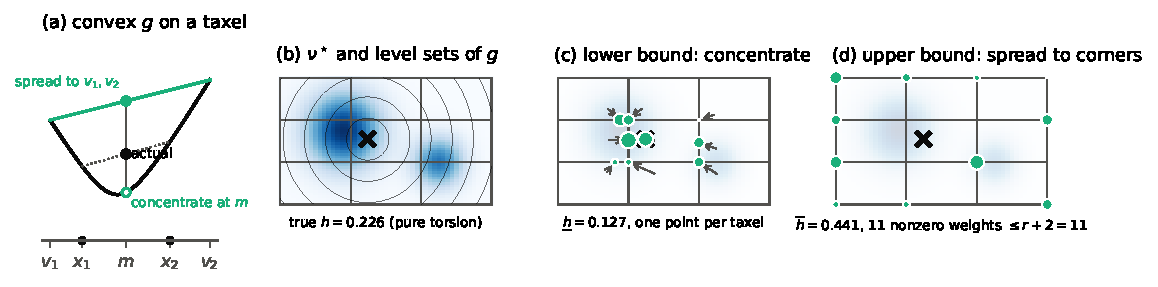
\includegraphics[width=\textwidth]{vertex_reduction}
    \caption{Concentrate vs.\ spread (Remark~\ref{rem:why_lemmas}), $3\times3$ taxels, pure torsion $q=(0,0,1)$, so $g(x;q,c)=\|x-c\|_2$.
    (a)~For masses at $x_1,x_2$ with CoP $m$: concentrating at $m$ lowers the objective (Jensen), spreading to the vertices
    $v_1,v_2$ raises it (chord). (b)~True measure and level sets of $g$. (c)~Minimizer of Theorem~\ref{thm:combined_lower}: one Dirac per
    taxel, pulled from the local CoPs of the taxels toward the CoP (arrows). (d)~Maximizer of Theorem~\ref{thm:combined_upper}: weights on the taxel
    corners, pushed away from the CoP, with at most $r+2$ nonzero weights. Marker areas are proportional to force.}
    \label{fig:vertex_reduction}
\end{figure}

\section{$\mathcal{M}_T$ case (taxel forces with CoP)}
\label{sec:MT}

\textit{Known:} the taxel forces $F_i$ and the CoP $c^\star=c[\nu_N^\star]$. \textit{Unknown:} the distribution of $\nu_N^\star$ inside each taxel.
Since $y_T$ determines the CoP, the set of compatible CoPs is reduced to a singleton $\mathcal C_{\mathcal M_T}(y_T)=\{c^\star\}$. Hence the outer optimization of
Lemma~\ref{lem:cop_slicing} disappears, and the $\mathcal M_T$-conditioned bounds reduce to the GMPs
\begin{align}
    \underline h_{\mathcal M_T}(q;y_T)
    =
    \inf_{\substack{
    \nu_N(P_i)=F_i,\ i=1,\ldots,r\\
    \int_P(x-c^\star)\,d\nu_N=0}}
    \mu\int_P
    \|a+bJ(x-c^\star)\|_2\,d\nu_N(x),
    \\
    \overline h_{\mathcal M_T}(q;y_T)
    =
    \sup_{\substack{
    \nu_N(P_i)=F_i,\ i=1,\ldots,r\\
    \int_P(x-c^\star)\,d\nu_N=0}}
    \mu\int_P
    \|a+bJ(x-c^\star)\|_2\,d\nu_N(x).
\end{align}
The taxel force constraints are disjoint, but the CoP consistency constraint $\int_P(x-c^\star)\,d\nu_N=0$ couples the measure $\nu_N$ across the taxels.
In what follows, $c$ denotes the measured CoP $c^\star$.

\begin{theorem}[Exact lower bound for combined measurements]
\label{thm:combined_lower}
    Under Assumption~\ref{ass:taxels}, given the combined observation $y_T=(y_0,y_F)$ with $y_0=(f_N,f_Nc)$ and $y_F=(F_1,\ldots,F_r)$,
    \begin{align}
        \label{eq:combined_lower_reduction}
        \boxed{\underline h_{\mathcal M_T}(q;y_T)
        =
        \mu
        \inf_{\substack{
            c_i\in P_i,\ i=1,\ldots,r\\
            \sum_{i=1}^rF_ic_i=f_Nc
        }}
        \sum_{i=1}^r
        F_i\left\|a+bJ(c_i-c)\right\|_2.}
    \end{align}
    This finite-dimensional problem is convex. \textcolor{red}{For polygonal taxels, it is an SOCP over the taxel closures? CHECK WITH YANN}.
\end{theorem}

\begin{theorem}[Exact upper bound for combined measurements]
\label{thm:combined_upper}
    Under Assumption~\ref{ass:taxels} with polygonal taxel closures $\overline{P_i}=\operatorname{conv}\{v_{i1},\ldots,v_{iK_i}\}$, for every $q=(a,b)\in\mathbb R^2\times\mathbb R$,
    \begin{align}
        \label{eq:combined_upper_reduction}
        \boxed{
        \begin{aligned}
        \overline h_{\mathcal M_T}(q;y_T)
        =
        \mu\max_{\lambda_{ik}\geq0}\quad&
        \sum_{i=1}^r\sum_{k=1}^{K_i}
        \lambda_{ik}
        \left\|a+bJ(v_{ik}-c)\right\|_2\\
        \text{subject to}\quad&
        \sum_{k=1}^{K_i}\lambda_{ik}=F_i,
        \qquad i=1,\ldots,r,\\
        &
        \sum_{i=1}^r\sum_{k=1}^{K_i}
        \lambda_{ik}v_{ik}=f_Nc.
        \end{aligned}}
    \end{align}
    This is a linear program. 
\end{theorem}

For a single taxel $P_1=P$, the constraint of \eqref{eq:combined_lower_reduction} forces $c_1=c$, and Theorem~\ref{thm:combined_lower} reduces to Theorem~\ref{thm:coarse_lower}.
Theorem~\ref{thm:combined_upper} reduces to Theorem~\ref{cor:coarse_upper_polygon}.

\paragraph{Cellwise bounds.}
Simpler, closed-form bounds are obtained by treating the taxels independently, dropping the coupling through the CoP.
For a reference point $c\in\R^2$ and $i=1,\ldots,r$, define
\begin{align}
g_i^{\min}(q;c)
\triangleq
\inf_{x\in P_i}
\|a+bJ(x-c)\|_2,
\qquad
g_i^{\max}(q;c)
\triangleq
\sup_{x\in P_i}
\|a+bJ(x-c)\|_2.
\end{align}
For $b\neq0$, with $p=c+Ja/b$, $g_i^{\min}(q;c)=|b|\operatorname{dist}(p,P_i)$ and, for polygonal closures, $g_i^{\max}(q;c)=|b|\max_k\|v_{ik}-p\|_2$. For $b=0$, both equal $\|a\|_2$.

\begin{proposition}[Constructive cellwise support bounds]
\label{prop:cellwise}
For every $q=(a,b)\in\mathbb R^2\times\mathbb R$,
\begin{align}
\label{eq:cellwise_MT}
\boxed{
\mu\sum_{i=1}^r F_i g_i^{\min}(q;c^\star)
\le
\underline h_{\mathcal M_T}(q;y_T)
\le
\overline h_{\mathcal M_T}(q;y_T)
\le
\mu\sum_{i=1}^r F_i g_i^{\max}(q;c^\star).
}
\end{align}
\end{proposition}
These cellwise bounds are directly computable from the taxel forces, the
measured CoP, and the taxel geometry, but need not be sharp: independently attaining the minimum or maximum within each taxel may violate
the global first-moment constraint contained in $\mathcal M_T$.

\section{$\mathcal{M}_F$ case (taxel forces without CoP)}
\label{sec:MF}

\textit{Known:} the taxel forces $F_i$. \textit{Unknown:} the CoP $c^\star$ and the distribution of $\nu_N^\star$ inside each taxel.
Contrary to $y_0$ and $y_T$, the taxel force measurement $y_F$ does not determine the CoP. It only confines it to the convex set
$\mathcal C_{\mathcal M_F}(y_F)$ of Proposition~\ref{prop:cop_taxel}, which shrinks as the taxel partition is refined. The bounds therefore keep the
bi-level structure of Lemma~\ref{lem:cop_slicing}, and the inner problems are exactly the $\mathcal M_T$ problems of Section~\ref{sec:MT}.

\begin{proposition}[$\mathcal M_F$ as $\mathcal M_T$ with unknown CoP]
\label{prop:MF_as_MT}
    For $c\in\mathcal C_{\mathcal M_F}(y_F)$, let $y_T(c)\triangleq((f_N,f_Nc),y_F)$. Then
    $\Pi_{\mathcal M_F}(y_F)=\bigcup_{c\in\mathcal C_{\mathcal M_F}(y_F)}\Pi_{\mathcal M_T}(y_T(c))$, and for every $q$,
    \begin{align}
        \label{eq:MF_as_MT}
        \boxed{
        \underline h_{\mathcal M_F}(q;y_F)=\inf_{c\in\mathcal C_{\mathcal M_F}(y_F)}\underline h_{\mathcal M_T}(q;y_T(c)),
        \qquad
        \overline h_{\mathcal M_F}(q;y_F)=\sup_{c\in\mathcal C_{\mathcal M_F}(y_F)}\overline h_{\mathcal M_T}(q;y_T(c)).}
    \end{align}
\end{proposition}

In practice, \eqref{eq:MF_as_MT} is an outer optimization over the known convex set $\mathcal C_{\mathcal M_F}(y_F)$ (a polygon for polygonal taxels).
Each inner problem is given by Theorem~\ref{thm:combined_lower} or~\ref{thm:combined_upper}. For the lower bound, the outer and inner minimizations merge into a single convex problem.

\begin{theorem}[Exact lower bound for taxel force measurements]
\label{thm:taxel_lower}
    Under Assumption~\ref{ass:taxels}, for every $q=(a,b)\in\mathbb R^2\times\mathbb R$,
    \begin{align}
        \label{eq:taxel_lower_reduction}
        \boxed{\underline h_{\mathcal M_F}(q;y_F)
        =
        \mu
        \inf_{\substack{c_i\in P_i\\i=1,\ldots,r}}
        \sum_{i=1}^r
        F_i\left\|a+bJ(c_i-\bar c)\right\|_2,
        \qquad
        \bar c
        \triangleq
        \frac{1}{f_N}\sum_{i=1}^r F_i c_i.}
    \end{align}
    This finite-dimensional problem is convex. \textcolor{red}{Is it simpler when taxels are polygonal?}
\end{theorem}

\begin{theorem}[Exact upper bound for polygonal taxels]
\label{thm:taxel_upper}
    Under Assumption~\ref{ass:taxels} with polygonal taxel closures, for weights $\lambda_{ik}\geq0$ with $\sum_{k=1}^{K_i}\lambda_{ik}=F_i$, let
    $\bar c(\lambda)\triangleq\frac{1}{f_N}\sum_{i=1}^r\sum_{k=1}^{K_i}\lambda_{ik}v_{ik}$. Then, for every $q=(a,b)\in\mathbb R^2\times\mathbb R$,
    \begin{align}
        \label{eq:taxel_upper_reduction}
        \boxed{\overline h_{\mathcal M_F}(q;y_F)
        =
        \mu
        \max_{\substack{
            \lambda_{ik}\geq0\\
            \sum_{k=1}^{K_i}\lambda_{ik}=F_i,\ \forall i
        }}
        \sum_{i=1}^r\sum_{k=1}^{K_i}
        \lambda_{ik}
        \left\|
        a+bJ\bigl(v_{ik}-\bar c(\lambda)\bigr)
        \right\|_2}
    \end{align}
\end{theorem}


\section{Comparison of measurements and tightening under refinement}
\label{sec:refinement}

The results of this section follow from Lemma~\ref{lem:monotone} (inclusion of compatible families) and from the fact that
$g(x;q,c)$ is $|b|$-Lipschitz in both $x$ and $c$.

\begin{proposition}[Comparison of coarse, taxel and combined measurements]
\label{prop:taxel_refinement}
The compatible measure family associated with the combined measurement is
$\Pi_{\mathcal M_T}(y_T)=\Pi_{\mathcal M_0}(y_0)\cap\Pi_{\mathcal M_F}(y_F)$.
Consequently, for every wrench direction $q\in\mathbb R^2\times\mathbb R$,
\begin{align}
\boxed{
\begin{aligned}
\mu f_N\|a\|_2
=
\underline h_{\mathcal M_0}(q;y_0)
\le
\underline h_{\mathcal M_F}(q;y_F)
\le
\underline h_{\mathcal M_T}(q;y_T)
&\le
h_{\mathcal W(\nu_N^\star)}(q),\\
h_{\mathcal W(\nu_N^\star)}(q)
\le
\overline h_{\mathcal M_T}(q;y_T)
&\le
\min\left\{
\overline h_{\mathcal M_0}(q;y_0),
\overline h_{\mathcal M_F}(q;y_F)
\right\}.
\end{aligned}
}
\end{align}
Thus, $\mathcal M_T$ provides bounds that are at least as tight as those
obtained from either $\mathcal M_0$ or $\mathcal M_F$ alone. The lower bounds of $\mathcal M_0$ and $\mathcal M_F$ are ordered,
whereas their upper bounds are not in general ordered.
\end{proposition}

\begin{proposition}[Tightening under taxel refinement]
\label{prop:taxel_refinement_MF}
If the taxel partition is refined (each $P_i$ is a union of finer cells $P_j'$), the compatible families and the compatible CoP set can only shrink.
Consequently, for $\mathcal M\in\{\mathcal M_F,\mathcal M_T\}$, with $\mathcal M'$ the refined measurement and $y=\mathcal M(\nu_N^\star)$, $y'=\mathcal M'(\nu_N^\star)$,
\begin{align}
\boxed{
\underline h_{\mathcal M}(q;y)
\le
\underline h_{\mathcal M'}(q;y')
\le
h_{\mathcal W(\nu_N^\star)}(q)
\le
\overline h_{\mathcal M'}(q;y')
\le
\overline h_{\mathcal M}(q;y).
}
\end{align}
\end{proposition}

The monotonicity above is associated with \textit{partition refinement}, not
with the number of taxels $r$ alone. The convergence below, on the other hand, only requires the taxel diameters to vanish.

\begin{proposition}[Resolution-dependent gap bounds]
\label{prop:taxel_resolution_MT}
For every $q=(a,b)\in\mathbb R^2\times\mathbb R$,
\begin{align}
\boxed{
\begin{aligned}
0
&\le
\overline h_{\mathcal M_T}(q;y_T)
-
\underline h_{\mathcal M_T}(q;y_T)
\le
\mu |b|
\sum_{i=1}^r
F_i\operatorname{diam}(P_i)
\le
\mu |b| f_N
\max_i\operatorname{diam}(P_i),\\
0
&\le
\overline h_{\mathcal M_F}(q;y_F)
-
\underline h_{\mathcal M_F}(q;y_F)
\le
2\mu |b|
\sum_{i=1}^r
F_i\operatorname{diam}(P_i)
\le
2\mu |b| f_N
\max_i\operatorname{diam}(P_i).
\end{aligned}
}
\end{align}
Hence, along any sequence of taxel partitions with
$\max_i\operatorname{diam}(P_i)\rightarrow0$, all four bounds converge to $h_{\mathcal W(\nu_N^\star)}(q)$.
\end{proposition}

\subsection{Current issues and open questions}

The three cases differ in the role played by the CoP. With $\mathcal M_0$ and
$\mathcal M_T$, the CoP is measured. The bounds are GMPs with explicit finite-dimensional forms: a convex lower bound and,
for polygonal taxels, an LP upper bound. With $\mathcal M_F$, the CoP is an unknown confined to the compatible set
$\mathcal C_{\mathcal M_F}(y_F)$, which contracts as the taxel partition is refined. The lower bound remains a single convex
program, but the upper bound requires a nonconvex outer search over $\mathcal C_{\mathcal M_F}(y_F)$ of $\mathcal M_T$ linear programs.
The main remaining questions concern
(i) efficient global solution of the $\mathcal M_F$ upper bound, i.e. the structure of $c\mapsto\overline h_{\mathcal M_T}(q;y_T(c))$;
(ii) the sharpness of the resolution-dependent bounds above (numerically, the gaps decrease linearly with $\max_i\operatorname{diam}(P_i)$, with constants below the bounds);
and (iii) the additional tightening provided by the CoP constraint in $\mathcal M_T$ relative to $\mathcal M_F$, which appears small in numerical experiments.

\begin{thebibliography}{9}

\bibitem{evans2015measure}
L.~C. Evans and R.~F. Gariepy,
\newblock \emph{Measure Theory and Fine Properties of Functions},
\newblock Revised ed., CRC Press, Boca Raton, FL, 2015.

\bibitem{lasserre2010moments}
J.-B. Lasserre,
\newblock \emph{Moments, Positive Polynomials and Their Applications},
\newblock Imperial College Press Optimization Series, vol.~1,
Imperial College Press, London, 2010.

\bibitem{winkler1988extreme}
G.~Winkler,
\newblock ``Extreme points of moment sets,''
\newblock \emph{Mathematics of Operations Research},
vol.~13, no.~4, pp.~581--587, 1988.

\end{thebibliography}
\end{document}
